
\epigraph{\textit{Dynamic programming is not about filling in tables. It's about smart recursion!}}{\citeauthor{algorithms_erickson}, \citeyear{algorithms_erickson} \cite{algorithms_erickson}}

%%%%%%%%%%%%%%%%%%%%%%%%%%%%%%%%%%%%%%%%%%%%%%%%%%%%%%%%%%%%%%
\subsubsection{Descripción de la solución recursiva}
Las funciones de coste funcionan de la misma manera que en el caso anterior, pero con la variación de que la función \texttt{transformar} utiliza programación dinámica para evaluar todas las posibles transformaciones en cada posición de las cadenas, almacenando los costos acumulados de cada subproblema en una matriz para evitar recalcular los mismos valores.

\subsubsection{Relación de recurrencia}
Este código utiliza programación dinámica para calcular el costo mínimo de transformar una cadena \texttt{s1} en otra \texttt{s2}. Para ello, utiliza una matriz \texttt{dp} donde \texttt{dp[i][j]} representa el costo mínimo para transformar los primeros \(i\) caracteres de \texttt{s1} en los primeros \(j\) caracteres de \texttt{s2}. Se definen costos para cuatro operaciones: sustitución, inserción, eliminación y transposición. La matriz se llena iterativamente, evaluando el costo mínimo entre estas operaciones. Al final, \texttt{dp[m][n]} contiene el costo mínimo de la transformación, que se imprime.

\subsubsection{Identificación de subproblemas}
El algoritmo identifica los subproblemas a resolver mediante la partición de las cadenas en segmentos más pequeños. Cada celda de la matriz \texttt{dp} corresponde a un subproblema que calcula el costo de transformar un prefijo de la cadena \texttt{s1} en un prefijo de la cadena \texttt{s2}. Estos subproblemas se resuelven de manera acumulativa, asegurando que los valores previamente calculados sean reutilizados en lugar de recalcularse.

\subsubsection{Estructura de datos y orden de cálculo}
El programa utiliza una matriz bidimensional \texttt{dp} de tamaño \( (m+1) \times (n+1) \), donde \(m\) y \(n\) son las longitudes de las cadenas \texttt{s1} y \texttt{s2}, respectivamente. El cálculo se realiza llenando esta matriz celda por celda, de izquierda a derecha y de arriba hacia abajo. Cada celda \texttt{dp[i][j]} se calcula considerando los costos de las operaciones posibles (sustitución, inserción, eliminación y transposición).

\subsubsection{Algoritmo utilizando programación dinámica}

\begin{itemize}
    \item Inicializa la matriz \texttt{dp} con dimensiones \( (m+1) \times (n+1) \).
    \item Llena la primera fila y la primera columna con valores base, correspondientes a los costos acumulados para transformar cadenas vacías.
    \item Itera sobre los índices \(i\) y \(j\) para calcular el costo mínimo en cada celda \texttt{dp[i][j]}, evaluando las operaciones de transformación.
    \item Al finalizar, el valor en \texttt{dp[m][n]} representa el costo mínimo de transformar \texttt{s1} en \texttt{s2}.
\end{itemize}

\begin{figure}[h]
    \centering
    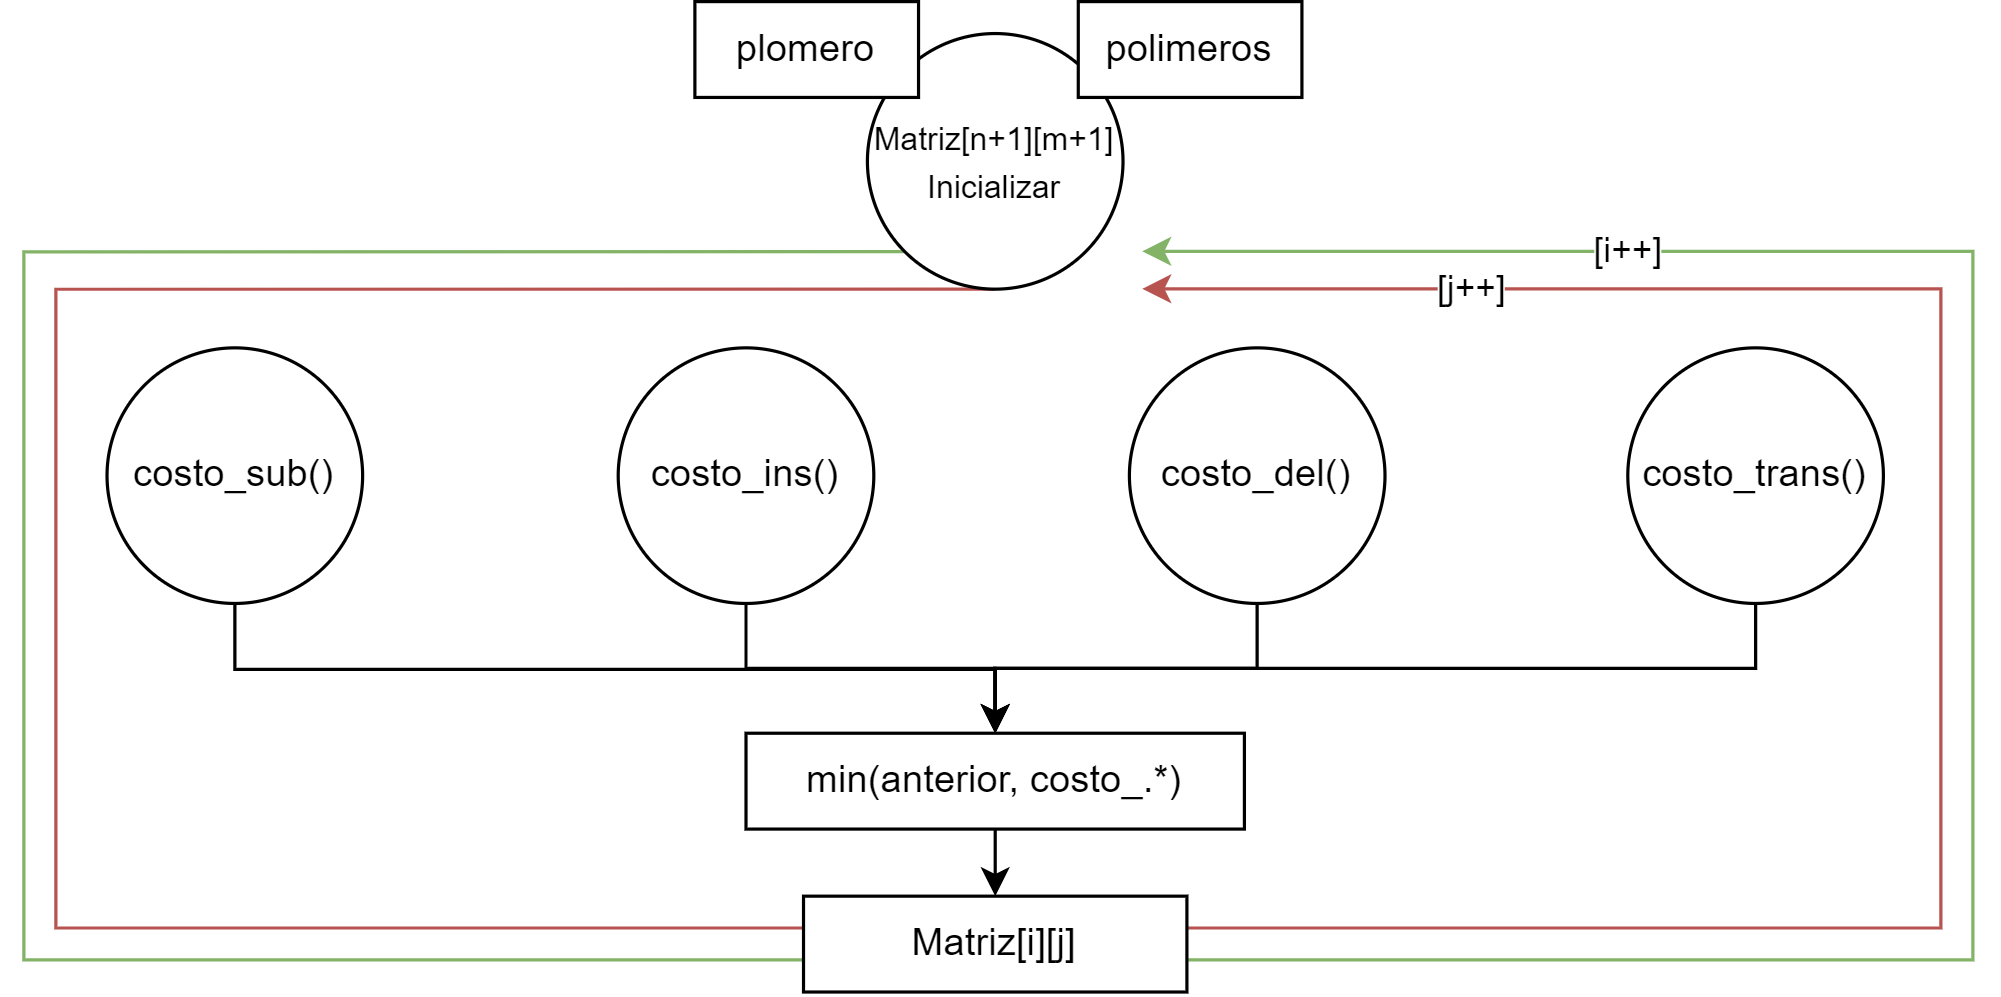
\includegraphics[width=.7\linewidth]{AlgoReportTemplate-main/images/DinamicProgramation.png}
    \caption{Visualización del proceso de programación dinámica.}
\end{figure}

\begin{figure}[h!]
    \centering
    \begin{minipage}{0.45\textwidth}
        \centering
        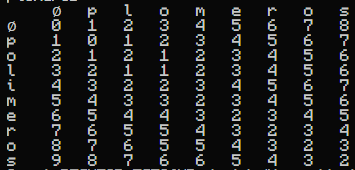
\includegraphics[width=1\linewidth]{AlgoReportTemplate-main/images/Matrix.png}
        \caption{Matriz resultante después de las iteraciones.}
    \end{minipage}%
    \hspace{1em}
    \begin{minipage}{0.45\textwidth}
        Después de completar las iteraciones necesarias, la matriz completa quedaría tal que así. Los valores corresponden al mínimo de la función de transformación, donde \texttt{dp[m][n]} es el valor óptimo.
    \end{minipage}
\end{figure}

\begin{algorithm}[H]
\SetKwProg{myproc}{Procedure}{}{}
    \SetKwFunction{Transformar}{Transformar}  % Cambia 'AlgorithmName' por el nombre del enfoque elegido
    \SetKwFunction{CostoSub}{costo\_sub}  % Función auxiliar de ejemplo
    \SetKwFunction{CostoIns}{costo\_ins}
    \SetKwFunction{CostoDel}{costo\_del}
    \SetKwFunction{CostoTrans}{costo\_trans}
    \DontPrintSemicolon
    \footnotesize

    % Definición del algoritmo principal
    \myproc{\Transformar{s1, s2}}{
    $m \leftarrow$ longitud de s1\;
    $n \leftarrow$ longitud de s2\;

    % Inicializar matriz dp con valores máximos
    Crear matriz $dp$ de tamaño $(m+1) \times (n+1)$ con todos los valores igual a $\infty$\;

    % Configurar condiciones iniciales
    $dp[0][0] \leftarrow 0$\;
    \For{$i \leftarrow 1$ \KwTo $m$}{
        $dp[i][0] \leftarrow dp[i-1][0] + \CostoDel{s1[i-1]}$\;  % Costo de eliminar caracteres de s1
    }
    \For{$j \leftarrow 1$ \KwTo $n$}{
        $dp[0][j] \leftarrow dp[0][j-1] + \CostoIns{s2[j-1]}$\;  % Costo de insertar caracteres de s2
    }

    % Llenar la matriz dp
    \For{$i \leftarrow 1$ \KwTo $m$}{
        \For{$j \leftarrow 1$ \KwTo $n$}{
            % Cálculo de sustitución
            $costo\_sust \leftarrow dp[i-1][j-1] + \CostoSub{s1[i-1], s2[j-1]}$\;
            $dp[i][j] \leftarrow \min(dp[i][j], costo\_sust)$\;

            % Cálculo de inserción
            $costo\_inser \leftarrow dp[i][j-1] + \CostoIns{s2[j-1]}$\;
            $dp[i][j] \leftarrow \min(dp[i][j], costo\_inser)$\;

            % Cálculo de eliminación
            $costo\_elim \leftarrow dp[i-1][j] + \CostoDel{s1[i-1]}$\;
            $dp[i][j] \leftarrow \min(dp[i][j], costo\_elim)$\;

            % Cálculo de transposición
            \uIf{$i > 1$ y $j > 1$ y $s1[i-1] = s2[j-2]$ y $s1[i-2] = s2[j-1]$}{
                $costo\_transp \leftarrow dp[i-2][j-2] + \CostoTrans{s1[i-2], s1[i-1]}$\;
                $dp[i][j] \leftarrow \min(dp[i][j], costo\_transp)$\;
            }
        }
    }

    \Return $dp[m][n]$\;  % Resultado final de la transformación mínima
}


    % Definición de la función auxiliar
    \myproc{\CostoSub{a, b}}{
    \Return \uIf{$a = b$}{0\;} \Else{2\;}
    }
    
    \myproc{\CostoIns{b}}{
        \Return 1\;
    }
    
    \myproc{\CostoDel{a}}{
        \Return 1\;
    }
    
    \myproc{\CostoTrans{a, b}}{
        \Return \uIf{$a = b$}{0\;} \Else{1\;}
    }
    \caption{Algoritmo basado en programación dinámica para calcular el costo mínimo de transformar una cadena \(s1\) en otra cadena \(s2\) mediante tabulacion.}
    \label{alg:mi_algoritmo_2}
\end{algorithm}

El programa tiene un orden temporal de \(O(m \times n)\), donde \(m\) y \(n\) son las longitudes de las cadenas. Esto se debe a que se llena una matriz de tamaño \( (m+1) \times (n+1) \), realizando un número constante de operaciones por celda para calcular los costos de las transformaciones posibles.

El algoritmo tiene un orden espacial de \(O(m \times n)\), ya que utiliza una matriz de tamaño \( (m+1) \times (n+1) \) para almacenar los resultados intermedios.

